\documentclass{beamer}
\usepackage{textcomp}
\usepackage{multimedia}
\usepackage{media9}

\usetheme{Rochester}
\usecolortheme{crane}

\definecolor{umber}{HTML}{A3C9F4}
\definecolor{light}{HTML}{DBECFF}

\setbeamercolor{frametitle}{fg=black, bg=umber}

\setbeamercolor{block body example}{bg=light}
\setbeamercolor{block title example}{bg=umber}


\setbeamercolor{frametitle}{fg=black}
\setbeamercolor{title}{fg=black, bg=umber}

\begin{document}

  \title[Crisis] % (optional, only for long titles)
  {Migration and Segregation in Three Dimensional Cellular Co-cultures}
  \subtitle{Role of Differential Cell Adhesion and Elasticity}
  \author[Author, Kolbman] % (optional, for multiple authors)
  {Dan Kolbman\\Mentor: Moumita Das}
  \date[2014]
  {Capstone I, Fall 2014}
  \subject{info}

  \frame{\titlepage}


  % MOVIES %
  \begin{frame}
    \frametitle{Experimental Motivation: Difference in physical properties of cells in a cell co-culture influence cell migration }
    \framesubtitle{}

	  \begin{columns}[t]
      \column{.5\textwidth}
      \begin{figure}
        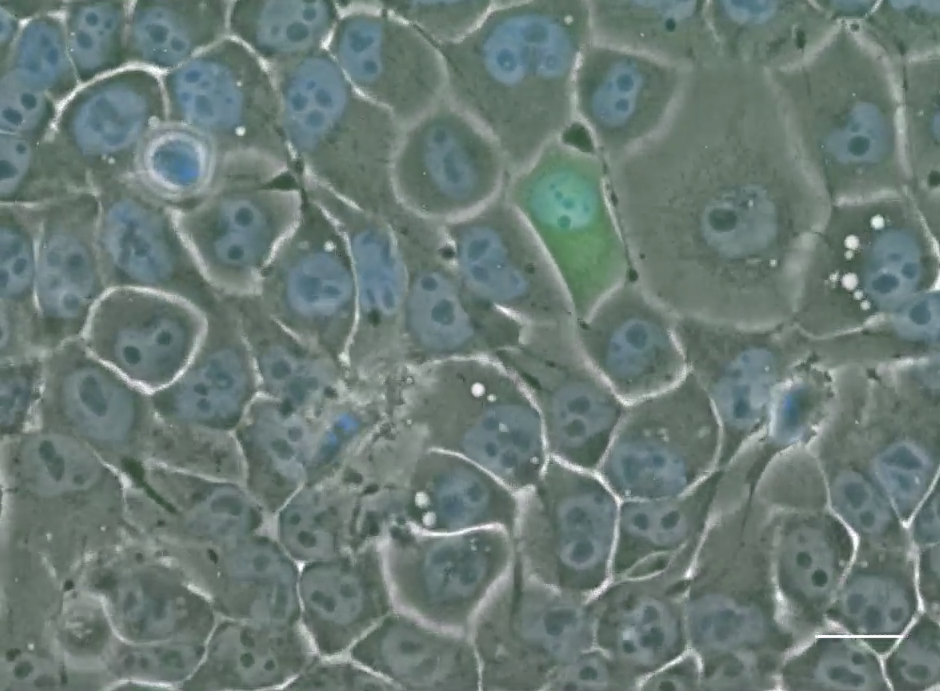
\includegraphics[width=1.0\textwidth]{cancercancer.png}
        \caption{Cancer cells}
      \end{figure}
      \column{.5\textwidth}
      \begin{figure}
        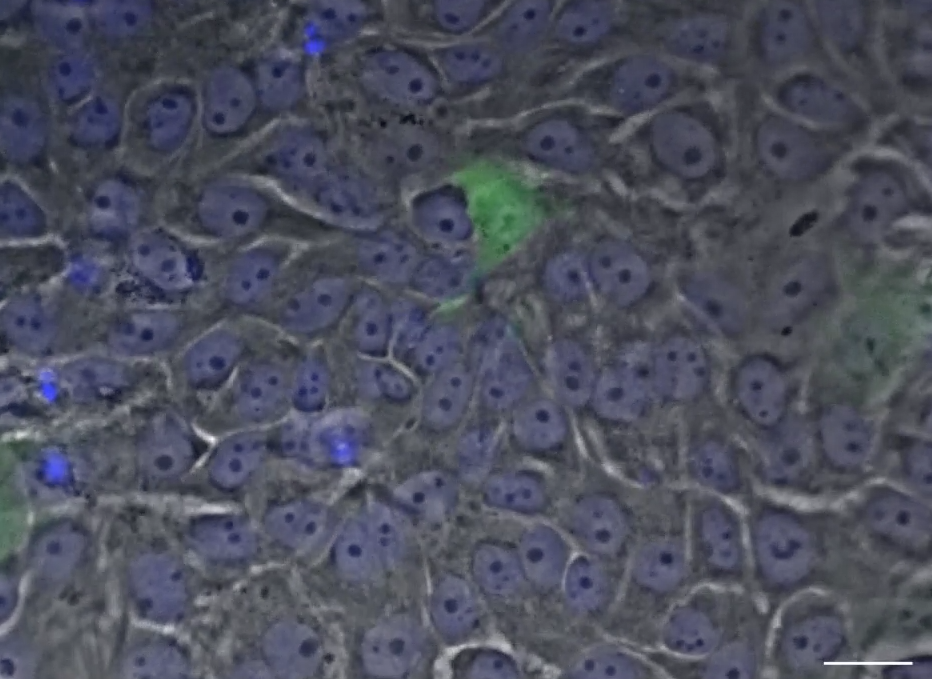
\includegraphics[width=1.0\textwidth]{cancerhealthy.png}
        \caption{Cancer cell in healthy cells}
      \end{figure}
    \end{columns}
    \footnote{From Wirtz Lab, Johns Hopkins. Biophysical Journal (2012). Used with permission of authors.}
    \vfill
    
  \end{frame}  
  
    % EXPERIMENTAL %
  \begin{frame}
    \frametitle{Experimental Motivation}
    \framesubtitle{Cell segregation in a co-culture of breast cancer cells and healthy breast epithelial cells.}
    \begin{figure}
    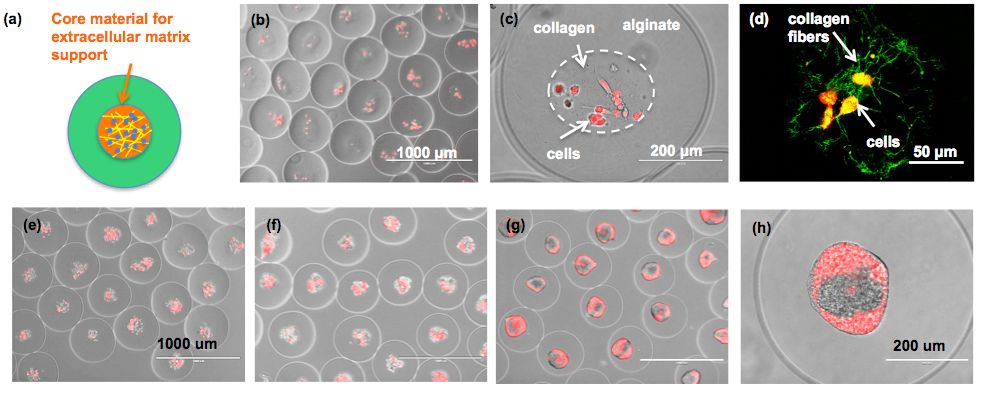
\includegraphics[width=1.0\textwidth]{experimental.png} \footnote{From M. Ma Lab, Cornell University. Used with permission of authors}
    \end{figure}

    \vfill
  \end{frame}
  
  % BACKGROUND %
  % Provide background about the subject. Talk about the different physical propreties %
  % and how they're thought to affect cancer migration and segregation %
  \begin{frame}
    \frametitle{Goal: To understand and predict the role of differential physical properties of cells in co-cultures}
              
 %\framesubtitle{Minimal ingredients of a model based on cell biophysical properties}
    
  \begin{itemize}    
    \item Cells are Brownian particles
    \item Cells are soft
    \item Cells are active and propel themselves
    \item Some cells show cell-cell adhesion
    \item A model cell co-culture consists of two (or more) types of cells all growing in one in vitro compartment.
  \end {itemize} 
          
  \vfill
    
  \end{frame}  
  

  % MODEL %
  % Discuss the general langevin equation for the dynamics of the system %
  \begin{frame}
    \frametitle{A proof of concept model}
    
    We study a confined binary system of active and deformable particles in 3D.
        
  \begin{exampleblock}{Over Damped Langevin Equation}
	  $$\vec{F}(\vec{r _m}) - \gamma \frac{d\vec{r_m}}{dt} + \vec{\eta}(t) = 0$$
	\end{exampleblock}
	\begin{columns}[t]
    \column{.5\textwidth}
      $\vec{F}$ -- Total force on the cell \\
      $\gamma$ -- The damping coefficient \\
      $\vec{r_m}$ -- Particle position. \\
    \column{.5\textwidth}
      $\vec{\eta}$ -- Fluctuating force due to activity and thermal fluctuations \\
  \end{columns}

  \vfill
    
  Model investigation in 2D co-cultures yielded promising results. (Butcher et al. unpublished).

  \end{frame}

  % INTERACTION FORCES %
  \begin{frame}
    \frametitle{Forces of the cells}
  	\begin{columns}[t] 
    % Initial system state %
  	\column{0.6\textwidth}
    \begin{figure}
      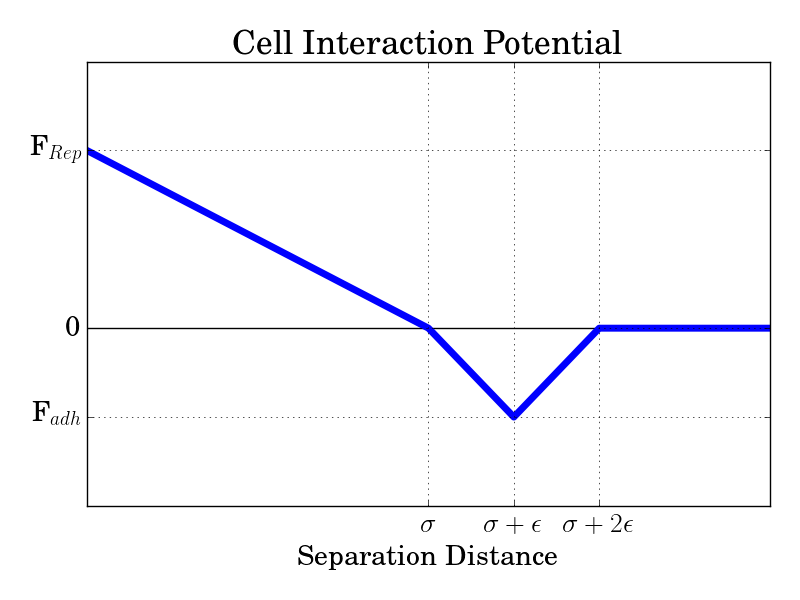
\includegraphics[width=1.0\columnwidth]{interaction.png}
%      \caption{Interaction Force}
    \end{figure}
    \column{0.4\textwidth}
    Three types of forces on the cells:
    \begin{itemize}
    \item Active forces generated by consumption of energy by cells. (Only cancerous cells)
    \item Elastic repulsion when cells push each other. 
    \item Cell-cell adhesion when cells come into contact. (Only healthy cells)
    \end{itemize}
    \end{columns}
    \vfill
  \end{frame}

  % BROWNIAN RESULTS %
  \begin{frame}
    \frametitle{Brownian Motion in 3D}
    %\framesubtitle{Brownian motion in 3D}
  	\begin{columns}[t] 
  	\column{0.6\textwidth}
  	\begin{figure}[h]
  	  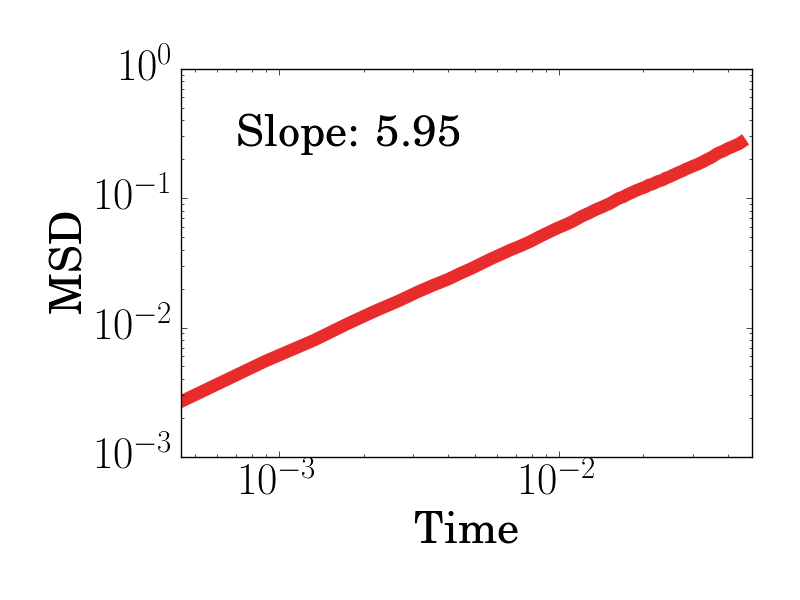
\includegraphics[width=2.5in]{brownianMSD.png}
      \caption{Mean Square Displacement (MSD) for a brownian system}
  	\end{figure}
    \column{.4\textwidth}
      \vspace{0.25in}
      \\
      For a 3D brownian system, Einstein says that: \\
      \begin{centering}
        $\bar{r^2} = 6Dt$ \\
      \end{centering}
      Where:\\
      $\bar{r^2}$ is the mean square displacement \\
      $D$ is the diffusion constant.
    \end{columns}
    \vfill
  \end{frame}

  % CO-CULTURE SYSTEM: MOTILITY %
  \begin{frame}
    \frametitle{A Co-Culture System in Our Model}
    \framesubtitle{Cell motility}
  	\begin{columns}[t] 
  	\column{0.6\textwidth}
  	\begin{figure}[h]
  	  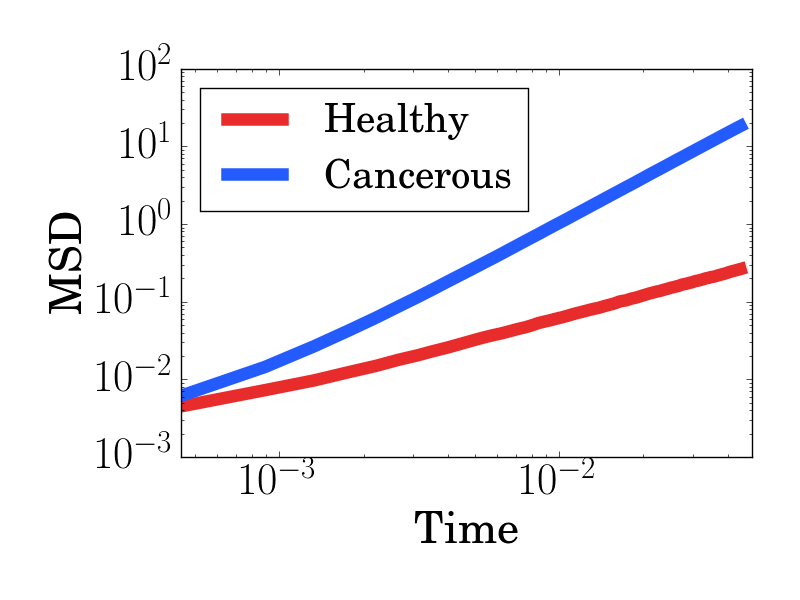
\includegraphics[width=2.5in]{cocultureMSD.png}
  	\end{figure}
    \column{.4\textwidth}
      \vspace{0.25in} \\
      \begin{itemize}
      \item Set the repulsion of healthy cells to 10x that of cancerous \\
      \item Give only cancer cells propulsion \\
      \item Give only healthy cells adhesion (Cancer cells don't have E-Cadherin)
      \end{itemize}
    \end{columns}
    \vfill
  \end{frame}

  % CO-CULTURE SYSTEM: SEPARATION %
  \begin{frame}
    \frametitle{A Co-Culture System in Our Model}
    \framesubtitle{Cell separation}
    \begin{figure}
  	  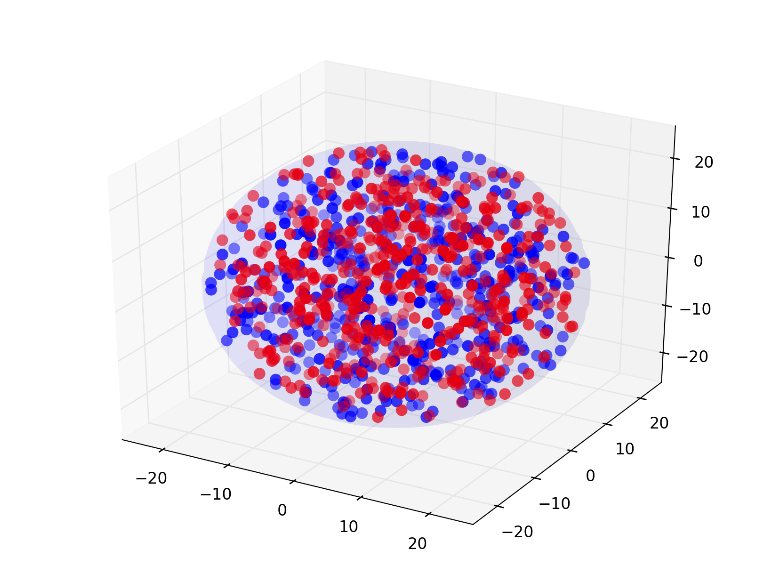
\includegraphics[width=0.75\textwidth]{3dconf.png}
      \caption{Separation in our 3D model}
    \end{figure}
    \vfill
  \end{frame}
  
  % FUTURE GOALS %
  \begin{frame}
    \frametitle{Future Goals in Capstone II}
    \framesubtitle{}

    \begin{itemize}\itemsep1pt \parskip0pt
      \item Apply experimental values and compare
      \item Add extra cellular matrix
      \item Add cell division (mitosis)
      \item Obtain results and analyze and interpreted  data
      \item Attend March Meeting and present results
      \item Calculate phase diagram with experimentally relevant parameters
      \item Write paper, give talk
    \end{itemize}
    
    \vfill
  \end{frame}
  
  % THANKS %
  \begin{frame}
    \frametitle{}
    \framesubtitle{}

    \centering{\Huge{Thanks!}} \\
    \vspace{0.5in}
    Dr. Das and Julian Butcher \\
    Dr. Barton and the Capstone Committee \\
    Drs Ma and Wu
    
    \vfill
  \end{frame}
  
    
\end{document}
